%
% main.tex -- Paper zum Thema <thema>
%
% (c) 2018 Nicolas Tobler, Hochschule Rapperswil
%

\chapter{Klima auf anderen Planeten\label{chapter:thema}}
\lhead{Klima auf anderen Planeten}
\begin{refsection}
\chapterauthor{Nicolas Tobler}

\section{Einleitung}

\rhead{Einleitung}
\begin{figure}
	% https://www.astrobio.net/news-exclusive/comparing-climates-from-earth-to-exoplanets/
	\centering
	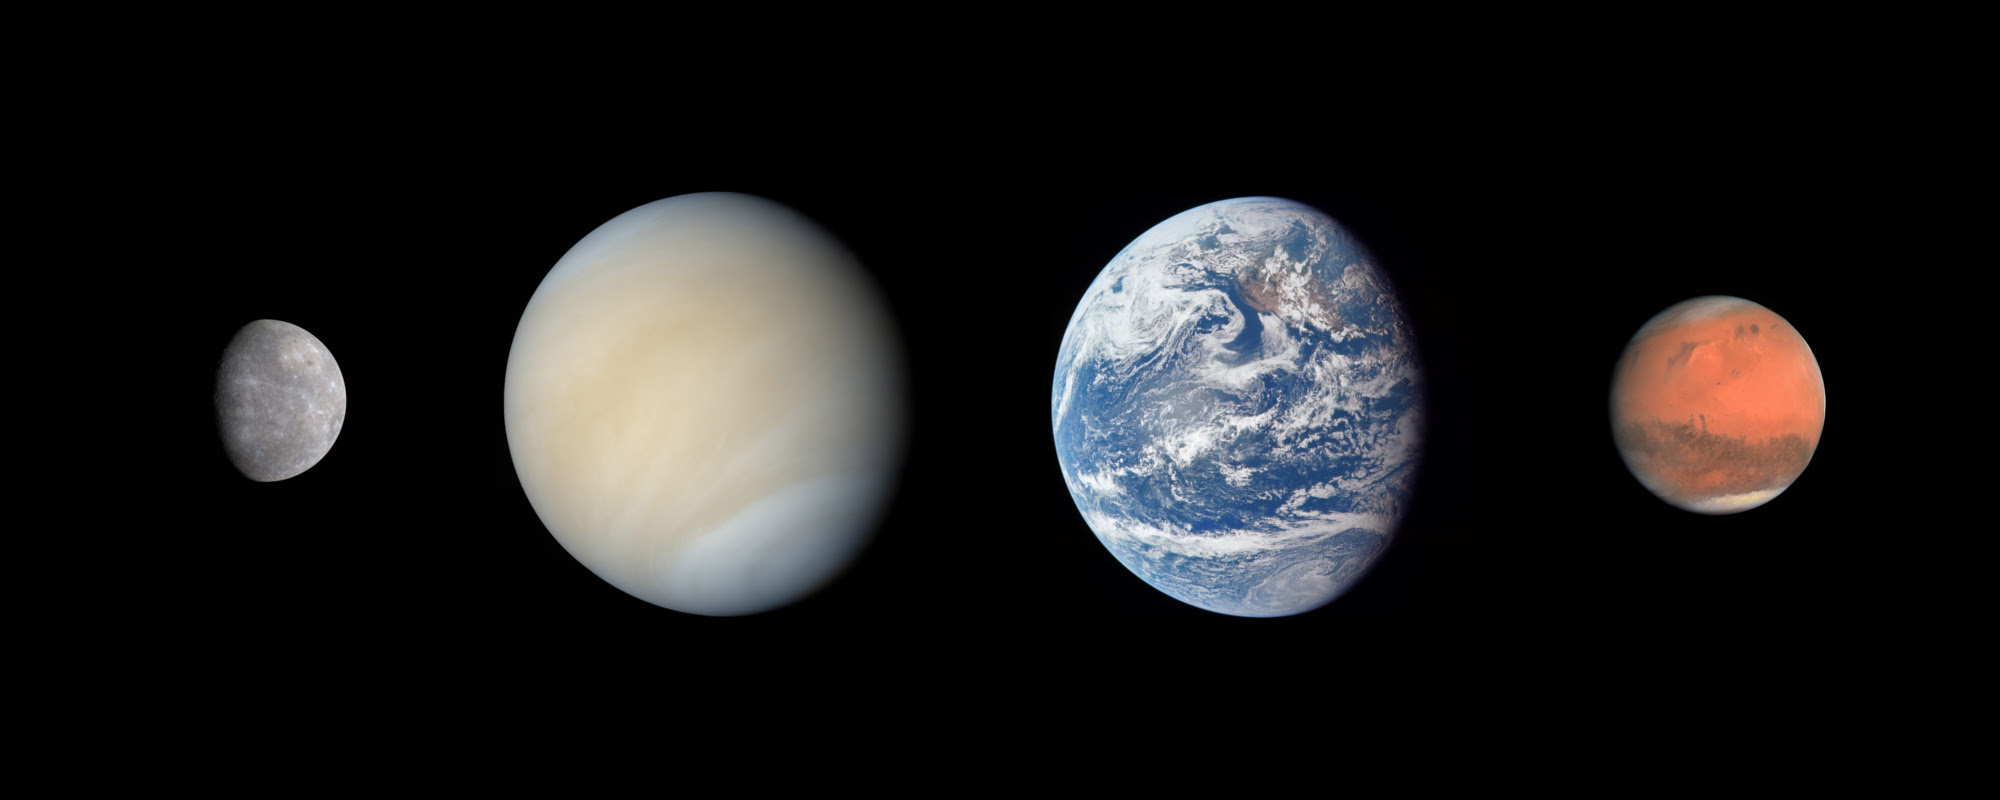
\includegraphics[width=0.7\linewidth, trim={0 2cm 0 2cm},clip]{planeten/Pictures/planets2.jpg}
	\caption{Merkur, Venus, Erde und Mars massstabsgerecht}
	% https://www.universetoday.com/13969/color-of-mercury/
	% https://medium.com/planet-stories/whats-false-about-true-color-2951ea5a4b5a
	% http://www.planetary.org/blogs/emily-lakdawalla/2009/2105.html
	% https://upload.wikimedia.org/wikipedia/commons/0/02/OSIRIS_Mars_true_color.jpg
\end{figure}

\begin{center}
\begin{table}
	\center
	\begin{tabular}{l|c c c c}
                           & Merkur         & Venus           & Erde    & Mars                  \\
  \hline
  Oberflächen Temperatur   & 452 K          & 733 K           & 287 K   & 226 K                 \\
  Wolken                   & -              & $\approx100\%$  & $68\%$  & $<5\%$                \\
  Atmosphäre               & $10^{-15}$ bar & $92$ bar        & $1$ bar & $6 \cdot 10^{-3}$ bar 
	%\hline
\end{tabular}
% (http://www.climate4you.com/ClimateAndClouds.htm) not used yet
\caption{Planeten im Vergleich}
\end{table}
\end{center}

%Verschiedene Organisationen, wie unter anderem Elon Musk's SpaceX, haben sich zum Ziel gemacht, in absehbarer Zukunft den Mars für den Menschen bewohnbar zu machen. Insbesondere sollte der Mars eine erdählnliche Atmosphere erhalte, also terraformed werden. Was auf Computer-generierten bildern ziemlich simpel aussieht, wird sich in realität wahrscheinlich ziemlich schwierig herausstellen. In diesem Kapitel wird die aktuelle lage des Klimas auf dem Mars analysiert und mögliche Wege den Mars zu teraformen auf die Machbarkeit untersucht.

Betrachtet man die vier der Sonne am nächst stehenden Planeten Merkur, Venus, Erde und Mars, gibt es einige Dinge festzustellen.
%Leben, wasser
Die Erde ist aus heutiger Sicht der einzige Planet der leben aufweist. Das für Leben notwendige flüssige Wasser ist auch nur auf der Erde in grossen Mengen auffindbar. Glücklicherweise lässt das, im Vergleich zu den anderen Planeten, milde Klima einen aktiven Wasserkreislauf zu. Alle anderen Planeten erfuhren offenbar ein anderes Schicksal. Falls auf ihnen je Wasser bestand, entwich es ins All oder gefror unter der Oberfläche. Das dortige Klima hat sich anders entwickelt.
%Temperatur
Man könnte meinen, dass primär die Distanz der Planeten zur Sonne für deren Temperatur ausschlaggebend ist. Jedoch nimmt die Temperatur über die Planeten mit der Entfernung zur Sonne nicht stetig ab. Das Klima muss somit auch von anderen Parametern abhängig sein, wie zum Beispiel Durchmesser, Rotation, Vulkanismus, Magnetfeld und viele andere. Obwohl Venus und Mars 

%Auf Venus, Erde und Mars kann flüssiges Wasser auftreten (Godilooks-Zone).
%Trotzdem sind neben der Erde auch Venus und Mars in der Godilooks-Zone, dem Gürtel um die Sonne, in welchem flüssiges Wasser auftreten kann.

Ein extremes Klima kann auch dazu führen, dass ein Planet sich irreversibel verändert, indem er zum Beispiel seine Atmosphäre ins All verliert. Wie es vermutlich beim Mars der Fall war. Trotz allen Einwirkungen sind wir in der glücklichen Lage auf der Erde ein mildes Klima vorzufinden, das Leben ermöglicht. Der Astrobiologe David Grinspoon ist folgender Meinung:

%TODO quote syntax?
\vspace{5pt}
\textit{“It may be that conditions for life’s origin aren’t rare, but the hard part is the persistence of habitable conditions.”} \\
\rightline{--- David Grinspoon, Astrobiologe \cite{planeten:AstrobiologyMagazine}}
%% https://www.space.com/21234-alien-planets-earth-climate-future.html
\vspace{5pt}

In diesem Kapitel gehe ich der Frage nach, ob Venus und Mars alleine aufgrund ihrer orbitalen Eigenschaften nicht fähig waren, ein lebensfreundliches Klima zu generieren. Die Nullhypothese lautet somit, dass die genannten Planeten \textit{nicht} durch ihre Umlaufbahn oder Grösse benachteiligt sind, Lebensfreundliche Klimabedingungen zu halten.

%Könnte es der Erde in Zukunft auch gleichermassen ergehen?
%Was führt zu wasserlosen Atmosphäre?

%Merkur ist in der Tabelle vertreten um zu verdeutlichen, dass nahe an der Sonne nicht direkt eine heisse Mitteltemperatur bedeutet.

\section{Ziel}
Es soll ein Modell erstellt werden, welches das Klima von Planeten mit deren orbitalen Eigenschaften verknüpft.
Betrachtet wird ein früher Zeitpunkt der Geschichte des Sonnensystems, als die Planeten ähnliche oder annähernd gleiche materielle und Atmosphärische Eigenschaften aufwiesen.
Mit der Annahme, dass grosse Mengen an Wasser auf allen Planeten vorhanden war, besteht auf allen Planeten die gleichen Voraussetzungen für mögliches Leben.
Das gleiche Modell wird mit unterschiedlichen orbitalen Parameter angewendet. Mann kann sich das vorstellen, als nehme man zum Beispiel die Erde, skaliert sie auf Mars-Grösse und setzt sie in den Mars-Orbit. 
Durch eine Simulation des Modells im Zeitbereich sollte dann eine Aussage über den Werdegang der Planeten gemacht werden.

%Dadurch kann der Werdegang der Planeten nachvollzieht werden.

%\subsection{Idee}
%Planeten mit gleichem Modell simulieren
%Orbitale Eigenschaften verwenden


%\subsection{Atmosphereische Eigenschaften}
%
%dünne Atmosphere
%
%Wann und wieso verlor der Mars seine Atmosphäre
%
%Rückgang der Atmosphäre durch Sonnenwind
%	https://www.nasa.gov/press-release/nasa-mission-reveals-speed-of-solar-wind-stripping-martian-atmosphere

\section{Modell}
\rhead{Modell}


	%Das Modell muss einige Sachen erfüllen, um eine Aussage machen zu können.
	
	%Das Modell wird so allgemein gehalten um für alle Planeten 

	%1. Für alle Planeten geltendes Modell erstellen
	
	%2. Modell soll 
	
	
	Das hier erarbeitete Modell muss für alle untersuchen Planeten gelten. Deshalb konzentriert es sich nur auf die Strahlungsbillanz und den Wasserkreislauf. Es wird davon ausgegangen, dass das Wasser signifikant für das Klima ist, da atmosphärischer Wasserdampf auf der Erde den grössten Anteil zum Treibhauseffekt beisteuert. Ausserdem befinden sich alle betrachteten Planeten in der Habitablen Zone, auch Bekannt als Goldilocks Zone. Diese beschreibt den Abstandsbereich um die Sonne, in dem flüssiges Wasser dauerhaft auftreten kann.
	Andere klimabestimmenden atmosphärischen Gase wie $\text{CO}_\text{2}$ werden nicht simuliert, um das Modell im gegebenen Rahmen umzusetzen.
	Das Modell sollte erdähnliche Bedingungen bewusst erstreben, um zu sehen ob diese auf den Planeten Mars und Venus auch bestehen können.
Auf Grund der zum Teil starken Vereinfachungen müssen einzelne Parameter abgeschätzt werden. Durch diese freien Parametern kann das System getrimmt werden um überhaupt plausible Lösungen zu erreichen. Diese Parameter sind mit $\xi$'s gekennzeichnet.
	Abbildung \ref{planeten:model} zeigt eine Übersicht des Modells. Die einzelnen Bestandteile werden im Folgenden beschrieben.

%Des Weiteren ist es für den Menschen interessant Planeten mit Erdähnlichen Zuständen anzutreffen.

%Zusammengefasst:

%Dazu müssen einige Annahmen getroffen werden:
%\begin{itemize}
%	\item Gleiche materielle Eigenschaften
%	\item Gleiches Vorkommen an Wasser
%	\item Wasser hat grösste Auswirkung auf Klima
%\end{itemize}			
	

%Möglichst auf einfachen Physikalischen Gesetzen basieren.	
	

\begin{figure}
	\centering
	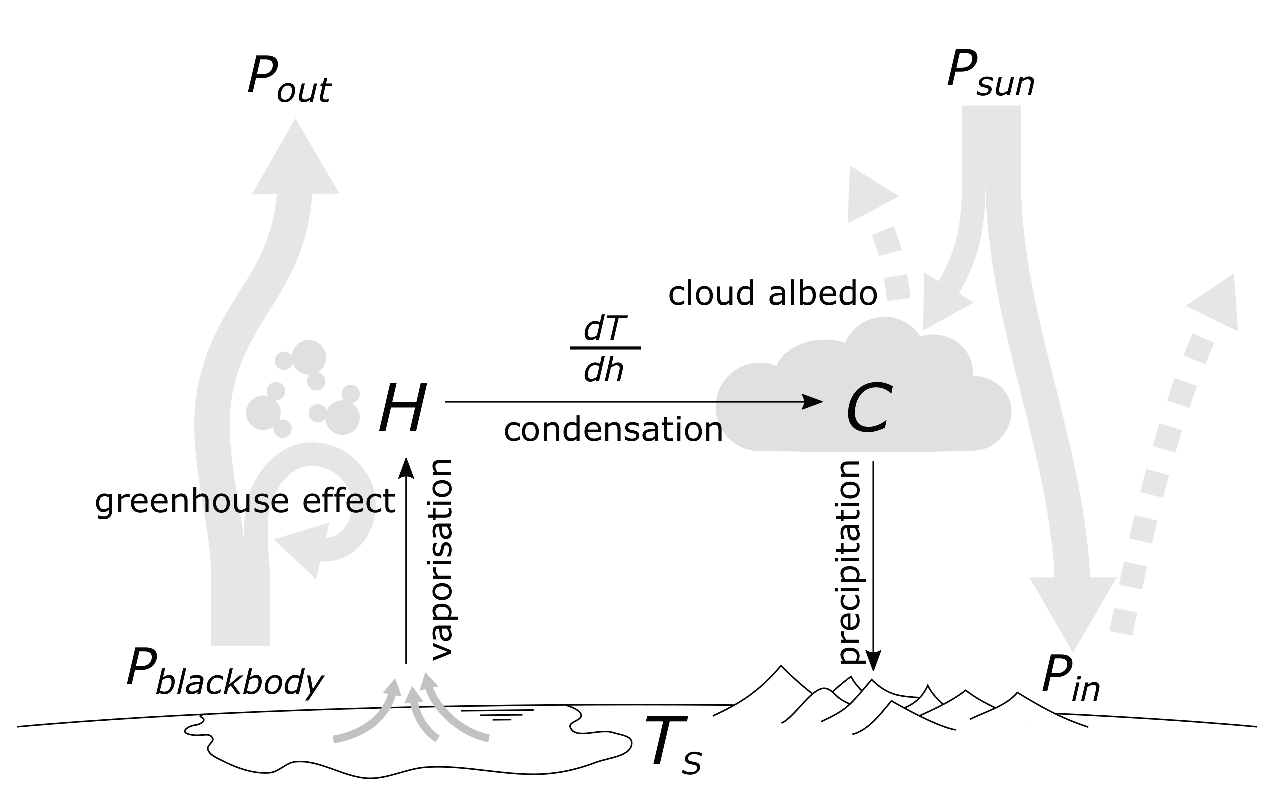
\includegraphics[width=0.8\textwidth]{planeten/Pictures/Model.eps}
	\caption{Modell-Übersicht}
	\label{planeten:model}
\end{figure}

\subsection{Strahlungsbilanz}
%TODO reference
Die Strahlungsbillanz wird in Kapitel \ref{skript:grundlagen:strahlung} ausführlich beschrieben. Das hier verwendeten Modell baut direkt darauf auf.

Damit die Durchschnittstemperatur eines Planeten stabil ist, muss die Leistungsbilanz Null sein.
\begin{equation}
\dot{T_S} \propto P_{\text{in}} - P_{\text{out}}
\end{equation}
Die Planeten sind jedoch nicht gleich gross. Damit die Auswirkung eines Strahlungsungleichgewicht für alle Planeten gleich ist, muss die Leistung auf eine Flächeneinheit normalisiert werden. Somit hat eine Stück Fläche mit der Atmosphäre darüber auf jedem Planeten die gleiche Wärmekapazität.
\begin{equation}
\dot{T_S} = \xi_1 \frac{P_{\text{in}} - P_{\text{out}}}{A} = \xi_1 \frac{P_{\text{in}} - P_{\text{out}}}{4 \pi R_{\text{planet}}^2}
\end{equation}

%TODO anderer begriff für Aktives Planet-Inneres .. geothermie? (nur für erde)
Die Eintreffende Leistung $P_{\text{in}}$ besteht primär aus der absorbierten Sonnenstrahlung. Andere Energiequellen wie ein Aktives Planet-Inneres und die Energie aus Gezeiten wird vernachlässigt. Es gilt:
%TODO P oder S für leistung pro fläche
\begin{equation}
P_{\text{in}} = \sigma T_{\astrosun}^4 \left( \frac{R_{\astrosun}}{a_{\text{planet}}} \right) ^2 \cdot (1-\alpha)
\end{equation}
Dabei ist $\alpha$ die Albedo des Planeten.

Dabei ist $\sigma$ die Stefan-Boltzmann-Konstante, $T_{\astrosun}$ \& $R_{\astrosun}$ die Oberflächentemperatur und Radius der Sonne, $ A_{\text{planet}}$ die mittlere Distanz des Planeten zur Sonne und $\alpha$ die Albedo des Planeten.

Die Abgestrahlte Leistung besteht praktisch ausschliesslich aus der Black-body Strahlung, welche sich aus der Durchschnittstemperatur $T$ und dem Radius $R_{\text{planet}}$ des Planeten bestimmen lässt. Diese Leistung bleibt jedoch teilweise durch den Treibhauseffekt in der Atmosphäre gefangen. Es gilt: 

\begin{equation}
P_{\text{out}} = 4 \pi R_{\text{planet}}^2 \sigma T_{S}^4 \epsilon
\end{equation}
Dabei ist $\epsilon$ der Anteil der durchdringenden Leistung.



\subsection{Albedo}

Die Albedo wird als Funktion der prozentualen Wolkenabdeckung $C$ modelliert. Es wird ein linearer Zusammenhang erwartet. Unter der Annahme, dass bei allen Planeten die Oberflächenalbedo $\alpha_{S}$ gleich ist, wird noch eine maximale Albedo $\alpha_{max}$ definiert. Bei 100\% Wolkendeckung soll der Maximalwert erreicht werden und bei 0\% die Oberflächenalbedo.

\begin{equation}
\alpha = \alpha_S + C(\alpha_{\text{max}} - \alpha_S)
\end{equation}

Die minimale Albedo entspricht etwa jeder des Mondes, der kleinsten in unserem Sonnensystem. Die maximale Albedo wird etwas grösser als diejenige der Venus gesetzt.
\begin{equation}
\alpha_S = 0.15, \alpha_{max} = 0.7
\end{equation}

\subsection{Treibhauseffekt}

Wasserdampf ist ein sehr effektives Treibhausgas. Es wird angenommen dass der atmosphärische Wasserdampf der Erde für 60\% des Treibhauseffekts sorgt.  
% 60\%    % https://www.acs.org/content/acs/en/climatescience/climatesciencenarratives/its-water-vapor-not-the-co2.html 
Im verwendeten Modell wirkt sich deren Konzentrazion $H$ linear auf den Teibhauseffekt $\beta$ aus. Die Wirkung wird mit $\xi_8$ beschränkt und kann vor der Simulation justiert werden.

\begin{equation}
\epsilon  = (1 - \beta) = (1 - \xi_8 \cdot H)
\end{equation}

\begin{equation}
\dot{T_S} = \xi_1 \frac{\sigma T_{\astrosun}^4 R_{\astrosun}^2}{4 \pi R_{\text{planet}}^2 a_{\text{planet}}^2} (\alpha_S + C(\alpha_{\text{max}} - \alpha_S)) - \xi_1 \sigma T_{S}^4  (1 - \xi_8 \cdot H)
\end{equation}

\subsection{Wasserkreislauf}

Das Modell beinhaltet einen stark vereinfachten Wasserkreislauf. Dieser besteht aus den zwei Boxen atmosphärischer Wasserdampf $H$ und Wolken $C$. Beides sind prozentuale Grössen und können näherungsweise als relative Luftfeuchtigkeit beziehungsweise prozentuale Wolkenabdeckung interpretiert werden. Dazu kommt das auf der Planetenoberfläche vorhandene flüssige Wasser, welches als Quelle und Senke dient und zugleich unerschöpflich ist. Das Modell beachtet nicht, dass der atmosphärische Wasserdampf ins All entweichen kann und dadurch die Ozeane austrocknen können.

%Dieser Prozess ist auf der Erde sehr komplex.

%\subsubsection{Wasserdampfbildung}
Wasserdampf bildet sich durch Verdunsten von der Ozeane. Der Durchsatz wird linear zur Oberflächentemperatur $T_S$ angenommen.
\begin{equation}
\xi_2 T_S
\end{equation}
%TODO linear zur temperatur !! überall kontrollieren

%\subsubsection{Wolkenbildung}

Wolken entstehen wenn feuchte Luft beim aufsteigen sich abkühlt und kondensiert. Näherungswiese entstehen mehr Wolken je grösser die Luftfeuchtigkeit $H$ ist und je schneller die Temperatur mit der Höhe abnimmt.
Dabei nimmt die Wolkenbildung mit grösserer Luftfeuchtigkeit $H$ und grösserem Temperaturgradienten $\frac{dT}{dh}$ zu. Durch Multiplizieren mit einem wählbaren Freiheitsgrad $\xi_3$ kann die Wirkung des Prozesses justiert werden. 
%Wolken bilden sich durch kondensieren des Wasserdampfs. Dieser Vorgang
%feuchte Luft abgekühlt wird
%bei grossem Temperaturgradienten
\begin{equation}
\xi_3 H \frac{dT}{dh}
\end{equation}

Wenn der Temperaturgradient linear Angenommen wird, lässt sich $\frac{dT}{dh}$ durch den Skalar $\Delta T $ vereinfachen.
Er existiert sowohl in vertikaler, sowie in horizontaler Ausrichtung. Einen grossen horizontalen Gradienten findet man bei einer Wetterfront vor. Im Modell wird nur der vertikale berücksichtigt. Dieser ist bei ungesättigter Luft annähernd konstant. Sobald Wasserdampf kondensiert wird der Prozess feuchtadiabatisch. Dabei wird der Gradient kleiner und sinkt mit zunehmender Temperatur noch weiter.
%TODO xi_10 neuen index zuweisen und andere anpassen.
Der Temperaturgradient sinkt bei 
\begin{equation}
\frac{dT}{dh} = \Delta T = \frac{\xi_9}{C T_S} 
\end{equation}

Eingesetzt erhält man für die Wolkenbildung:
\begin{equation}
\xi_3 H \frac{\xi_9}{C T_S}
\end{equation}

%\subsubsection{Wolkenabbau}
Wolken regnen, wenn sich die mikroskopischen Wassertropfen oder Eiskristalle verbinden und nicht mehr getragen werden können. Im hier verwendeten Modell wird angenommen, dass sich Regenbildung somit proportional zur Wolkenabdeckung $C$ verhält.
\begin{equation}
\xi_4 C
\end{equation}

%\subsection{Zusammengefasst}
%Der ganze Wasserkreislauf lässt sich somit durch folgendes Gleichungssystem zusammenfassen.
%
%\begin{equation}
%	\begin{matrix}			
%		\dot{H} = & \xi_2 P_{\text{in}}(C) & - \xi_3 H \Delta T & \\
%		\dot{C} = &                        &   \xi_3 H \Delta T & - \xi_4 C
%	\end{matrix}	
%\end{equation}


%\subsection{Entweichen von atmosphärischen Gasen}
%
%Ob ein Planet oder Mond eine Atmosphäre besitzt ist von wenigen parametern abhängig. Planeten behalten ihr Atmosphäre, wenn die Gravitation ausreichend stark ist, um die Moleküle gegen ihre thermische Geschwindigkeit zurückzuhalten.
%Die Moleküle in der Atmosphäre, für die
%
%% https://www.tcd.ie/Physics/people/Peter.Gallagher/lectures/PY4A03/pdfs/PY4A03_lecture12n13_amospheres.ppt.pdf
%
%\begin{equation}
%v_{escape} > v_{therm}
%\end{equation}
%
%zutrifft, werden nach und nach in den Weltraum abgestossen.
%Die Fluchtgeschwindigkeit eines Planeten $v_{escape}$ wird durch deren Masse $M$ und Radius $R$ berechnet: 
%
%\begin{equation}
%v_{escape} = \sqrt{\frac{2GM}{R}}
%\end{equation}
%
%wobei $G$ die Gravitationskonstante ist. Die Fluchtgeschwindigkeit ist somit bei grossen und schweeren Gestirnen grösser.
%
%Die thermische Geschwindigkeit eines Moleküls ist Maxwell-Bolzmann-verteilt. Deshalb gilt der berechnete Wert in diesem Zusammenhang nur approximativ. Die höchst wahrscheinliche Geschwindigkeit ist: 
%
%\begin{equation}
%v_{therm} = \sqrt{\frac{3kT}{m}}
%\end{equation}
%
%Dabei ist $k$ die Bolzmann-Konstante und $m$ die Mol-Masse des Moleküls. Die kritische Temperatur $T_{escape}$, bei welcher Gase abgestossen werden ist somit:
%
%\begin{equation}
%T_{escape} = \frac{2GMm}{3kR}
%\end{equation}

\subsection{Gleichungssystem}

Durch Zusammenfassen von Strahlungsbilanz und Wasserkreislauf erhält man folgendes Gleichungssystem:
\begin{equation}
\begin{matrix}
\dot{T_S} = & \xi_1 \frac{\sigma T_{\astrosun}^4 R_{\astrosun}^2}{4 \pi R_{\text{planet}}^2 a_{\text{planet}}^2} (\alpha_S + C(\alpha_{\text{max}} - \alpha_S)) && - \xi_1 \sigma T_{S}^4  (1 - \xi_8 \cdot H)\\
\dot{H}   = & \xi_2 T_S              & - \xi_3 H \frac{\xi_9}{C T_S}          & \\
\dot{C}   = &                        &   \xi_3 H \frac{\xi_9}{C T_S}          & - \xi_4 C
\end{matrix}
\end{equation}
Um zu verhindern, dass eine Luftfeuchtigkeit oder Wolkenabdeckung von über 100\% auftritt, werden zu gewissen linearen Termen noch den gleichen Term mit grosser Potenz dazu addiert. Somit wird der Effekt verstärkt wenn die Grösse nahe an $1$ also $100\%$ kommt. Das mit Anpassungen für gesättigten Wasserdampf und Wolkenabdeckung versehene Gleichungssystem lautet somit:
\begin{equation}
\begin{matrix}
\dot{T_S} = & \xi_1 \frac{\sigma T_{\astrosun}^4 R_{\astrosun}^2}{4 \pi R_{\text{planet}}^2 a_{\text{planet}}^2} (\alpha_S + C(\alpha_{\text{max}} - \alpha_S)) && - \xi_1 \sigma T_{S}^4  (1 - \xi_8 \cdot H)\\
\dot{H}   = & \xi_2 P_{\text{in}}(C) & - \xi_3 (H + H^9) \frac{\xi_9}{C T_S}   &                   \\
\dot{C}   = &                        &   \xi_3 (H + H^9) \frac{\xi_9}{C T_S}   & - \xi_4 (C + C^5)
\end{matrix}
\end{equation}

\section{Simulation}
\rhead{Simulation}

Das Modell wurde in MATLAB mittels Transientenanalyse simuliert. Dazu kam ein ODE45 Solver zur Hilfe. Die Anfangswerte wurden so gesetzt, dass sie Erdbedingungen unterstützen.  
%System anregen Erdähnliche Werte zu generieren.
\begin{equation}
\begin{matrix}
T_0 = & 287 \\
H_0 = & 0.44 \\
C_0 = & 0.68
\end{matrix}
\end{equation}
Die hinzugefügten Freiheitsgrade $\xi_1$ bis $\xi_6$ wurden empirisch gesetzt um für die Erde stabile Resultate zu erhalten.
%TODO why i picked those xi's
\begin{equation}
\begin{matrix}
\xi_1 = & 1                 \\
\xi_2 = & 1.5 \cdot 10^{-3} \\
\xi_3 = & 1.9 \cdot 10^{-2} \\
\xi_4 = & 4   \cdot 10^{-1} \\
\xi_8 = & 0.6
\end{matrix}
\end{equation}

In Tabelle \ref{planeten:planetValues} sind die für die Planeten eingesetzten Parameten $a_{\text{planet}}$ und $R_{\text{planet}}$ ersichtlich.
\begin{center}
\begin{table}
	\center
	\begin{tabular}{l|c c c c}
                        & Merkur                    & Venus                    & Erde                    & Mars     \\
  \hline
  $a_{\text{planet}}$   & $2.353 \cdot 10^{11}$ m   & $1.076 \cdot 10^{11}$ m  & $1.499 \cdot 10^{11}$ m & $2.353 \cdot 10^{11}$ m \\
  $R_{\text{planet}}$   & $3.3895 \cdot 10^{6}$ m   & $6.0519 \cdot 10^{6}$ m  & $6.371 \cdot 10^{6}$ m  & $3.3895 \cdot 10^{6}$ m 
\end{tabular}
\caption{Für die Planeten eingesetzte Werte aus WolframAlpha}
\label{planeten:planetValues}
\end{table}
\end{center}





Das System wurde bis zum stationären Zustand simuliert. Aus der Zeitachse können keine quantitative Schlüsse gezogen werden.

\subsection{Ergebnisse}

		Die Strich-Punkt-Linie der entsprechenden Farbe zeigt den heutigen Wert der Grösse. 

		\begin{figure}
			\center
			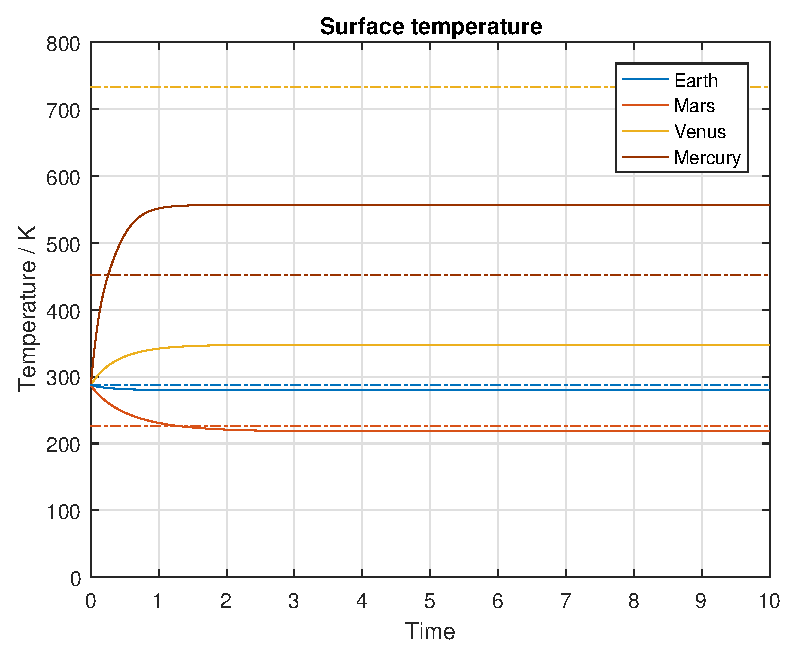
\includegraphics[height=0.45\textheight]{planeten/Matlab/figures/surfaceTemperature.eps}
			\caption{Globale Durchschnittstemperatur}
		\end{figure}
		
		\begin{figure}
			\center
			\includegraphics[height=0.45\textheight]{planeten/Matlab/figures/humidity.eps}
			\caption{Relative Luftfeuchtigkeit}
		\end{figure}
		
		\begin{figure}
			\center
			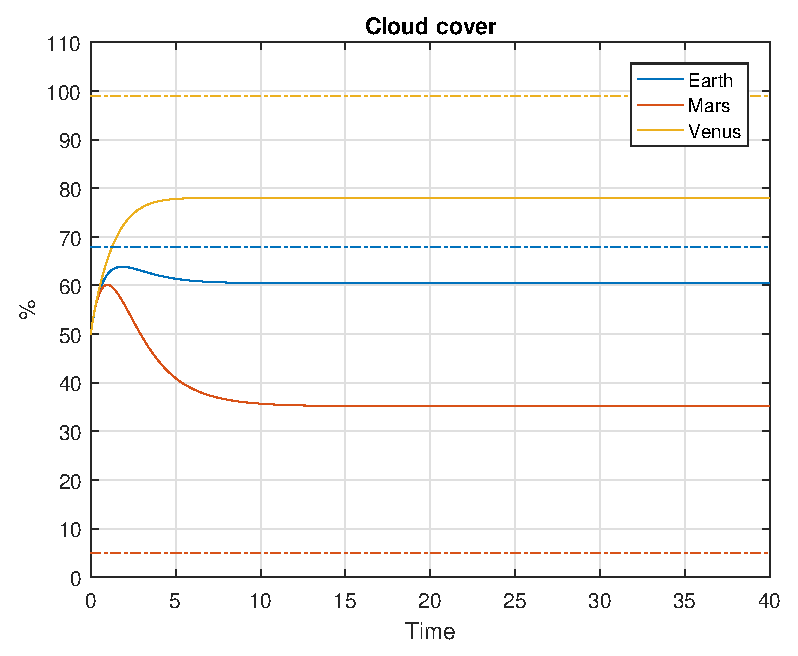
\includegraphics[height=0.45\textheight]{planeten/Matlab/figures/cloudCover.eps}
			\caption{Prozentuale Wolkenabdeckung}
		\end{figure}
		
		\begin{figure}
			\center
			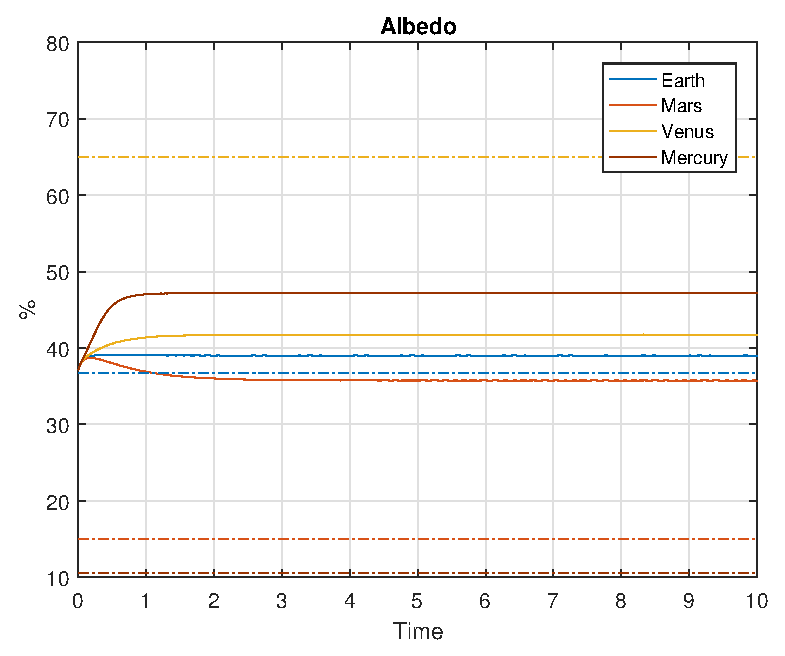
\includegraphics[height=0.45\textheight]{planeten/Matlab/figures/albedo.eps}
			\caption{Albedo}
		\end{figure}

\section{Schlussfolgerung}
\rhead{Schlussfolgerung}

Die Simulationsergebnisse tendieren zu den heutigen beobachtbaren Klimaverhältnisse. Die extremen Klima von Mars und Venus sind somit vermutlich durch ihre Grösse und Umlaufbahn prädestiniert. Die Nullhypothese kann somit falsifiziert werden. Es können jedoch nur qualitative Schlüsse gezogen werden, da durch Verändern der freien Parameter ein ganz anderes Bild entsteht. Somit sind die Ergebnisse nur mit Vorsicht zu geniessen.

Abweichungen sind durch diverse Fehlerquellen gerechtfertigt. Zum einen wurden diverse chemische und physikalische Vorgänge bei extremen Temperaturen und Sonneneinstrahlung nicht beachtet.
Neben Wasser wurden Treibhausgase wie CO$_2$ vernachlässigt. Sie machen heute den grössten Anteil der Venus- und Marsatmosphäre aus.

\subsection{Verbesserungsmöglichkeiten}

Dieses Modell bietet diverse Ausbaumöglichkeiten. Um zum Beispiel mehr Genauigkeit in den Extremen Bereichen zu erreichen, müssten mehr atmosphärische Gase einbezogen werden.
Diese Gase besitzen wiederum unterschiedliche Gefrierpunkte, was die Modellierung der Vereisung zulässt.
		
Im simulierten Modell wurden lediglich der Durchmesser und die Distanz zur Sonne der Planeten einbezogen. Um die Aussagekraft zu verbessern könnten weitere Planet-abhängige Parameter implementiert werden, wie der Vulkanismus und die Rotationsgeschwindigkeit. Die Rotation erlaubt das Modellieren von Tag- und Nachtseitentemperatur, welche sich stark auf das Klima auswirken.

\printbibliography[heading=subbibliography]
\end{refsection}
